\section{Analysis procedure}
This analysis note will describe in detail the analysis procedure to select events belonging to the $\gamma (p,n) \pi^+$ channel (See Fig. \ref{fig:frost_diagram}) from the g9a data set corresponding to the linearly polarised beam and longitudinally polarised target settings. Charged particles are identified with high efficiency in the CLAS detector ($\geq90\%$ \cite{Mecking2003}), so the analysis relies on detecting the $\pi^+$ and reconstructing the neutron from kinematics. The $\pi^+ n$ channel was first identified by filtering the data based on the invariant mass, beta and timing of each $\pi^+$ event. The neutron was then reconstructed using the missing mass technique. Neutral particles could only be detected with a much lower efficiency ($\sim5\%$ for neutrons with momenta $\sim 0.6 GeV/c$ increasing to $\sim 50\%$ for neutrons with momenta $\geq2 GeV/c$  \cite{Mecking2003}), which would significantly reduce the event sample. Once the channel of interest had been identified, the azimuthal ($\phi$) distribution of the $\pi^+$ in the CLAS detector was obtained, binned according to $\pi^+$ center-of-mass energy, W, and the cosine of the center-of-mass polar angle, $cos(\theta)$. The data set analysed  was divided into subsets for each photon beam (or coherent peak) energy setting (730, 930, 1100, 1300, 1500, 1700, 1900, 2100 and 2300 MeV) and for each target setting (target polarisation parallel or anti-parallel to the beam), providing in total 18 subsets (see Table \ref{tab:g9a_configs}) of data in the energy range 730-2300 MeV (W =1400-2290 MeV). At the binning stage, the data were also further subdivided according to the specific linear photon beam polarisation setting i.e. whether the electric field vector of the photon beam was parallel to the floor (PARA), perpendicular to the floor (PERP) or unpolarised (AMO). I will describe now the next stages of analysis, in which the G double-polarisation observable is extracted from the $\pi^+$ azimuthal distributions.
\begin{figure}[htb]
  \begin{center}
    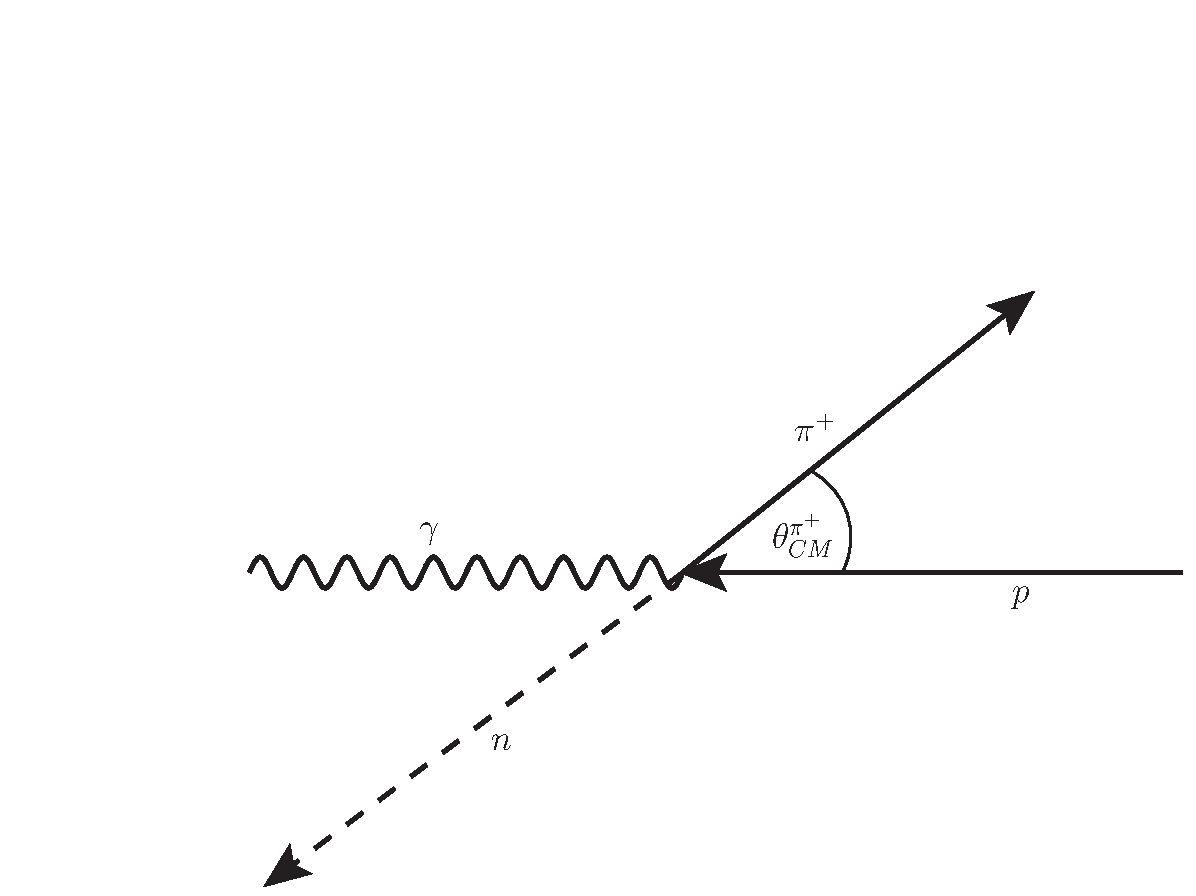
\includegraphics[width=0.6\textwidth]{figures/frost_reaction.pdf} \\
    \caption{The $\gamma p \rightarrow \pi^+ n $ reaction in the center of mass frame. }
    \label{fig:frost_diagram}
  \end{center}
\end{figure}

\begin{table}
  \begin{center}
    \begin{tabular}{ |l||l|l||l|l||l|l||l|l||}
      \hline
      \multicolumn{9}{|c|}{g9a Run period: Linearly polarized } \\
      \hline
      \multicolumn{3}{|l||}{$E_{beam}$} & \multicolumn{6}{|c||}{2.780 GeV}   \\
      \hline
      \multicolumn{3}{|l||}{$Coh_{Edge}$} & \multicolumn{2}{|c||}{0.73 GeV} &  \multicolumn{2}{|c||}{0.93 GeV} &  \multicolumn{2}{|c||}{1.1 GeV}   \\
      \hline
      \multicolumn{3}{|l||}{} & $E_{CMS}^{min} $ &  $E_{CMS}^{max} $ & $E_{CMS}^{min} $ &  $E_{CMS}^{max} $ & $E_{CMS}^{min} $ &  $E_{CMS}^{max} $\\
      \multicolumn{3}{|l||}{(GeV)} & 1.4 & 1.5 & 1.54 & 1.63 & 1.63 & 1.72  \\
      \hline
      \multicolumn{3}{|l||}{} & n  &  $\Delta E$ & n  &  $\Delta E$ & n  &  $\Delta E$ \\
      \multicolumn{3}{|l||}{(MeV)} & 4 & 25 & 3 & 30 & 3 & 30  \\
      \hline
      \hline
      $E_{beam}$&  \multicolumn{8}{|c||}{3.545 GeV} \\
      \hline
      $Coh_{Edge}$&  \multicolumn{2}{|c||}{1.1 GeV*} &  \multicolumn{2}{|c||}{1.3 GeV} &  \multicolumn{2}{|c||}{1.5 GeV} &  \multicolumn{2}{|c||}{1.7 GeV} \\
      \hline
      & $E_{CMS}^{min} $ &  $E_{CMS}^{max} $& $E_{CMS}^{min} $ &  $E_{CMS}^{max} $ & $E_{CMS}^{min} $ &  $E_{CMS}^{max} $ & $E_{CMS}^{min} $ &  $E_{CMS}^{max} $ \\
      (GeV) & 1.63 & 1.72 & 1.71 & 1.83 & 1.835 & 1.925 &  1.93 & 2.02 \\
      \hline
      & n  &  $\Delta E$ & n  &  $\Delta E$ & n  &  $\Delta E$& n  &  $\Delta E$ \\
      (MeV) & 3 & 30 & 4 & 30 & 3 & 30 &3 &30 \\
      \hline
      \hline
      \multicolumn{3}{|l||}{$E_{beam}$} &  \multicolumn{6}{|c||}{4.599 GeV} \\
      \hline
      \multicolumn{3}{|l||}{$Coh_{Edge}$} &  \multicolumn{2}{|c||}{1.9 GeV} &  \multicolumn{2}{|c||}{2.1 GeV} &  \multicolumn{2}{|c||}{2.3 GeV}  \\
      \hline
      \multicolumn{3}{|l||}{} & $E_{CMS}^{min} $ &  $E_{CMS}^{max} $& $E_{CMS}^{min} $ &  $E_{CMS}^{max} $ & $E_{CMS}^{min} $ &  $E_{CMS}^{max} $ \\
      \multicolumn{3}{|l||}{(GeV)} & 1.945 & 2.105 & 2.05 & 2.2 & 2.19 & 2.29 \\
      \hline
      \multicolumn{3}{|l||}{} & n  &  $\Delta E$ & n  &  $\Delta E$ & n  &  $\Delta E$ \\
      \multicolumn{3}{|l||}{(MeV)} & 4 & 40 & 3 & 50 & 2 & 50  \\
      \hline
    \end{tabular}
  \end{center}
  \caption{g9a Run period: Different electron beam energies ($E_{beam}$) were used with different Energies for the Coherent Edge Polarization ($Coh_{Edge}$). The photon energy profile has a direct correlation with the Center of Mass Energy ($E_{CMS}$), which was then binned in a range that assured enough statistics with a Beam Polarization $>50\%$ in order to avoid strong systematic error in the evaluation of the beam polarization. The range used in each configuration ($E_{CMS}^{min} $ ,  $E_{CMS}^{max}$), the number of bins (n) and the size of each bin is also shown in this table. For each setting were done independent measurements with different target polarizations. For $Coh_{Edge}$ settings of 1.1 GeV measurements were done with 2 different beam energies: The one denoted with (*) was not used, since the statistic for this setting ($E_{Beam}=3.545 GeV$, $Coh_{Edge}=1.1 GeV$) was considerably lower ($\sim \frac{1}{5}$) than in the other setting ($E_{Beam}=2.780 GeV$, $Coh_{Edge}=1.1 GeV$) and had just negative target polarization.} \label{tab:g9a_configs}
\end{table}

\subsection{Data Reduction}
The BOS files stored on the JLab tape silo contain all the data collected during CLAS JLab experiments. Before the analysis of these data could begin, a preliminary reduction of the g9a dataset was carried out allowing the reduced files to be copied to the Edinburgh work disks and to reduce the CPU time required for analysis. The CLAS analysis package, ROOTBEER \cite{rootbeer} was used for the preliminary data reduction process as well as for the subsequent analysis procedure described in this chapter. This is based on ROOT/C++ and interprets the bank structure of CLAS data. In this preliminary event selection two conditions determined the events which were retained:
\begin{enumerate}
\item  For each event, between one and three particles must be detected in conjunction with a hit in the tagger.
\item  Only three combinations of particles were allowed:
  \begin{enumerate}
  \item one positive particle,
  \item one positive and one neutral particle,
  \item one positive and two neutral particles.
  \end{enumerate}
\end{enumerate}
The resulting files were then output as more compact ROOTDST (Data Summary Tape) files.

\subsection{The g9a Targets}
In the g9a experiment there were three targets simultaneously in the beamline, as shown in Figure \ref{fig:target_draw}.
\begin{figure}[htb]
  \begin{center}
    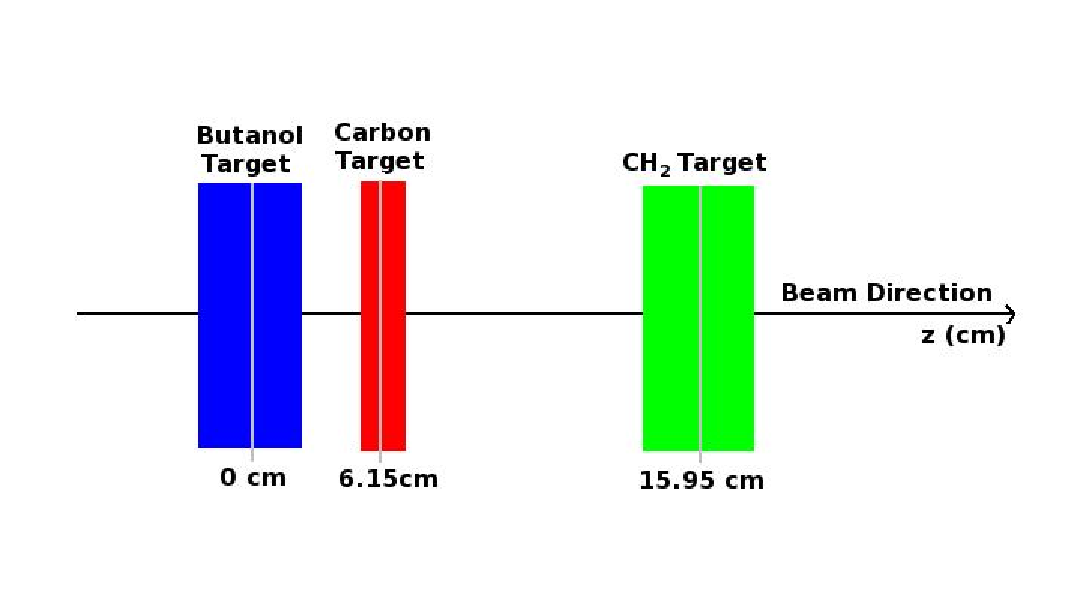
\includegraphics[width=0.6\textwidth]{figures/targets_drawing.png} \\
    \caption{Schematic diagram of the butanol, carbon and $CH_2$ targets in the beamline (not to scale) showing the position of their centers along the z-axis. }
    \label{fig:target_draw}
    \end{center}
  \end{figure}
The butanol ($C_4 H_9OH$) target formed part of the FROST target system,  providing polarised protons. As butanol contains unpolarised carbon and oxygen atoms as well as polarised hydrogen, analysis of events originating within the carbon target allowed assessment of this unpolarised background contribution. The $CH_2$ target provides unpolarised protons, another useful cross-check for the analysis. Events from each of the three targets were selected by making a cut on the z-vertex position of each event to originate within one of the three targets. The z-vertex position is defined as the point of intersection of the beamline axis with the particle’s trajectory extrapolated back from the drift chambers. Figure \ref{fig:target_pos} shows the z-vertex position of all positive particle events along with the cuts made on the target positions as follows: -2.67 cm $\leq$ z $\leq$ 2.67 cm for the butanol target, 5.0 cm $\leq$ z $\leq$ 7.0 cm for the carbon target and 15.0 cm $\leq$ z $\leq$ 17.0 cm for the $CH_2$ target.
\begin{figure}[!htb]
  \begin{center}
    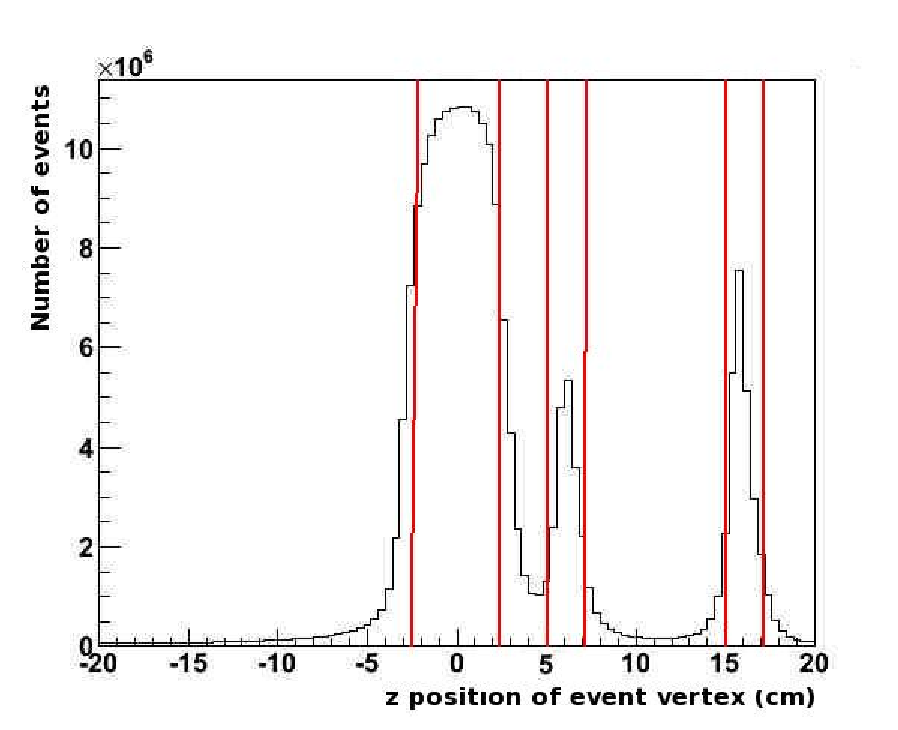
\includegraphics[width=0.6\textwidth]{figures/targets_pos.png} \\
    \caption{Z-vertex distribution of all positively charged particle events. The vertical red lines show the cuts made on the target positions as described in the text.}
    \label{fig:target_pos}
  \end{center}
\end{figure}



\subsection{Calculation of the Photon Beam Polarization}
To extract the G observable, as well as the other polarisation observables measured in this experiment, it was necessary to know the degree of linear beam polarisation as accurately as possible. The orientation of the polarisation plane must also be established with accuracy and can be determined from the goniometer settings. The calculation of the degree of linear beam polarisation involves comparing the shape of the coherent Bremsstrahlung spectrum to a spectrum obtained from theoretical Bremsstrahlung calculations. An enhancement plot can be used to separate the coherent contribution from the incoherent contribution to the spectra. The enhancement plots are fit with a theoretical spectrum produced by the Analytical Bremsstrahlung (ANB) Calculation \cite{Natter_2003}\cite{Sabin_2010}. The ANB calculation takes into account 17 experimental parameters characterizing the geometry of the radiator, collimator and photon beam. Several of these parameters can be measured experimentally (such as photon beam energy and beam spot size) whereas others (such as electron beam divergence on the radiator) are varied until a good agreement is obtained between the enhancement plot and the ANB calculation. These parameters are then extracted from the fit and are used to calculate the degree of polarisation per event as a function of photon energy. This information is then summarised in lookup tables \cite{Anderson_table}. For the g9a run period there was also some extra step. The Coherent Edge could not be re-calculated at the time of the analysis since the records from the tagger scaler (in the TESC bank) were not saved in the data stream. The best available option, after consulting with University of Glasgow experts, was relying on recorded EPICS data for the Coherent Edge position, data obtained and recorded at the time of data taking. Since EPICS records data after a short analysis on a small sample of data a double step procedure was done while analyzing the data:
\begin{enumerate}
\item run through the data and record the Coherent Edge position and the event number
\item Create a Tree data structure that connects to each event number a coherent edge position 
\end{enumerate}



\subsection{\texorpdfstring{$\pi^+$}{pi+} identification}
Different cuts were applied on the data in order to select events with a single $\pi^+$.
\begin{enumerate}
  \item number of photons in the same RF bucket = 1
  \item mass calculated from SC and TAG
  \item charge of track = +1
  \item The $\beta$ distribution was fitted for different momentum bins and a $\pm 3 \sigma$ cut was applied around the center of the distribution (see Fig. \ref{fig:beta_mom_pip} ) for particles with momentum $p_{\pi^+} < 1.2GeV$. For higher momentum, the statistic was poorer for clearly defining a $\pm 3 \sigma$ cut and no contamination was clearly seen in this range after all the cuts.
  \item  $\pm 3 \sigma$ cut around the $m^2$ of the pion (See Fig. \ref{fig:mass2_pip}).
\end{enumerate}
\begin{figure}[!htb]
  \begin{center}
    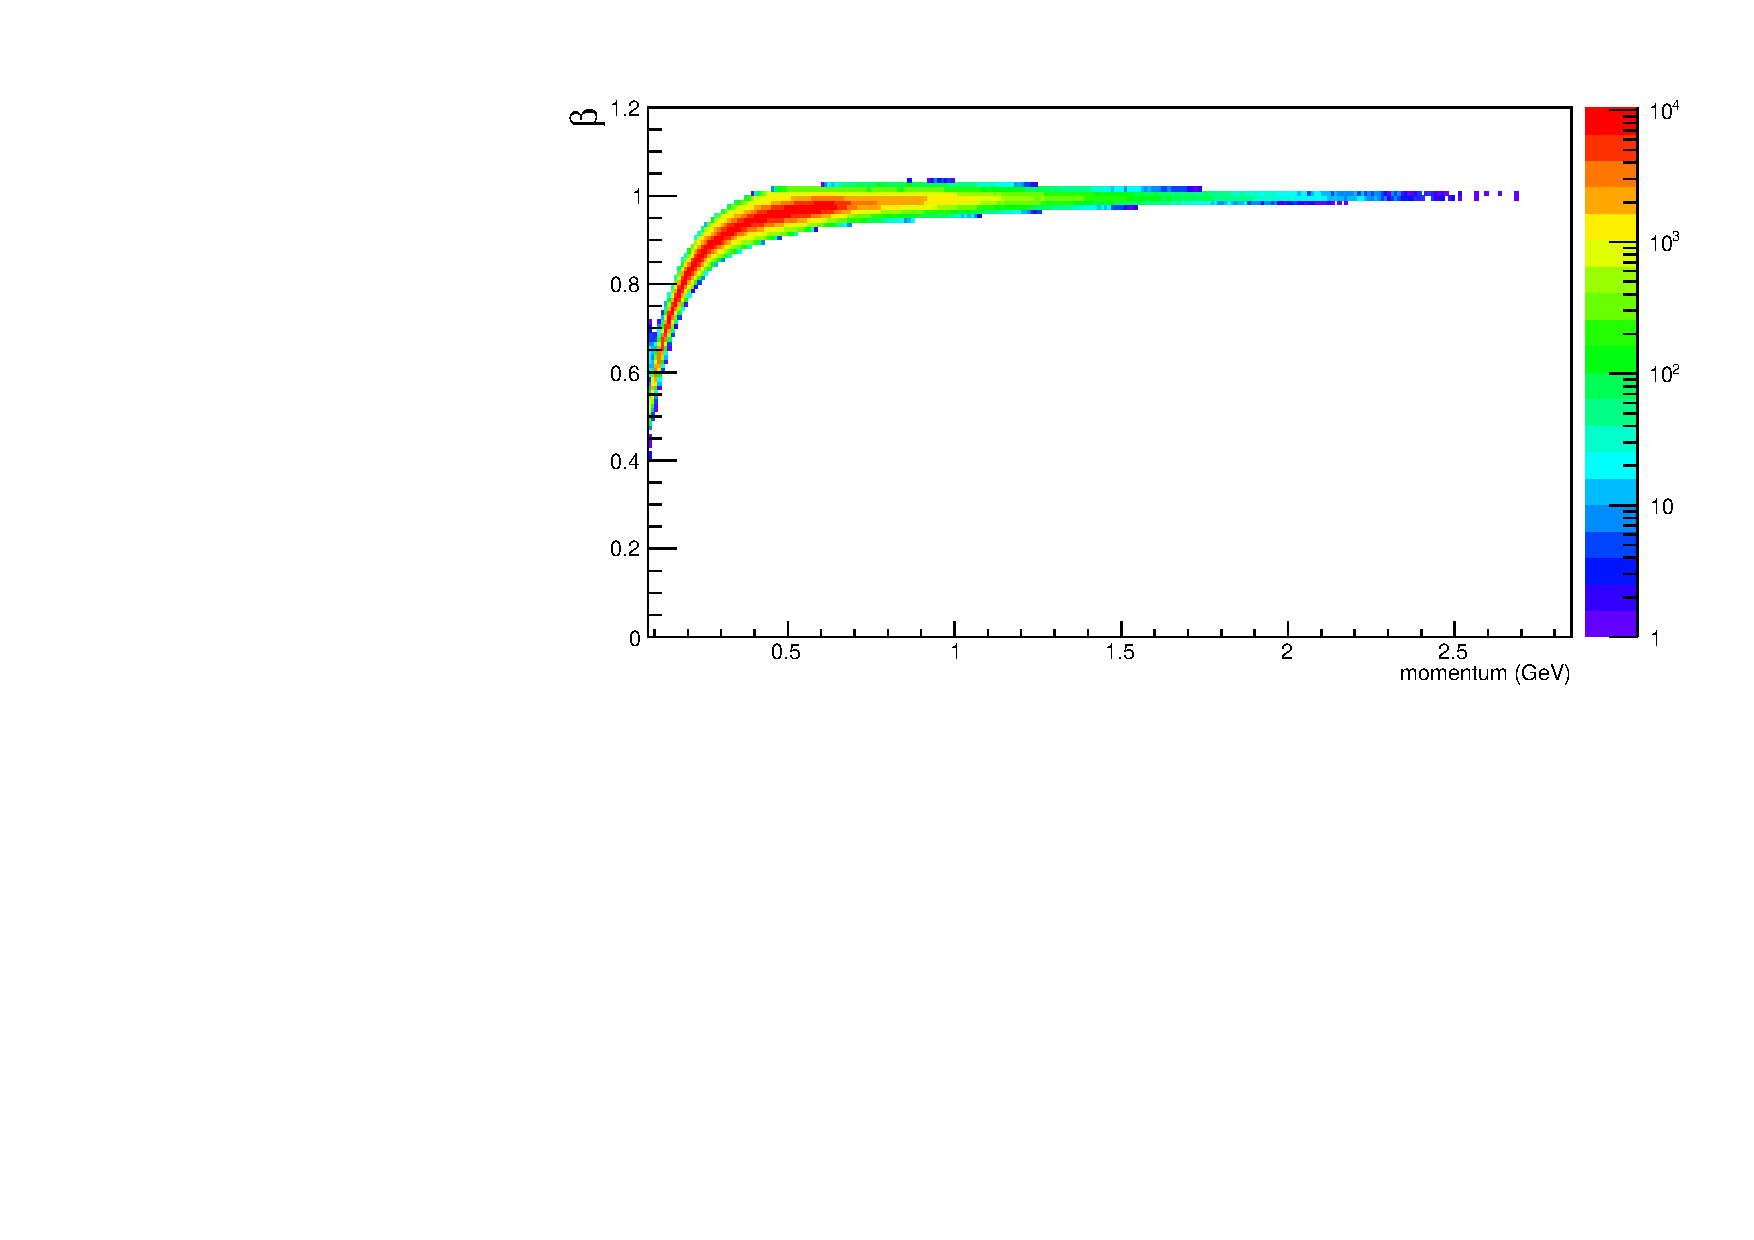
\includegraphics[width=0.6\textwidth]{figures/pid_beta_mom_pip.pdf} \\
    \caption{$\beta$ vs $momentum$ for the selected $\pi^+$ tracks}
    \label{fig:beta_mom_pip}
  \end{center}
\end{figure}
\begin{figure}[!htb]
  \begin{center}
    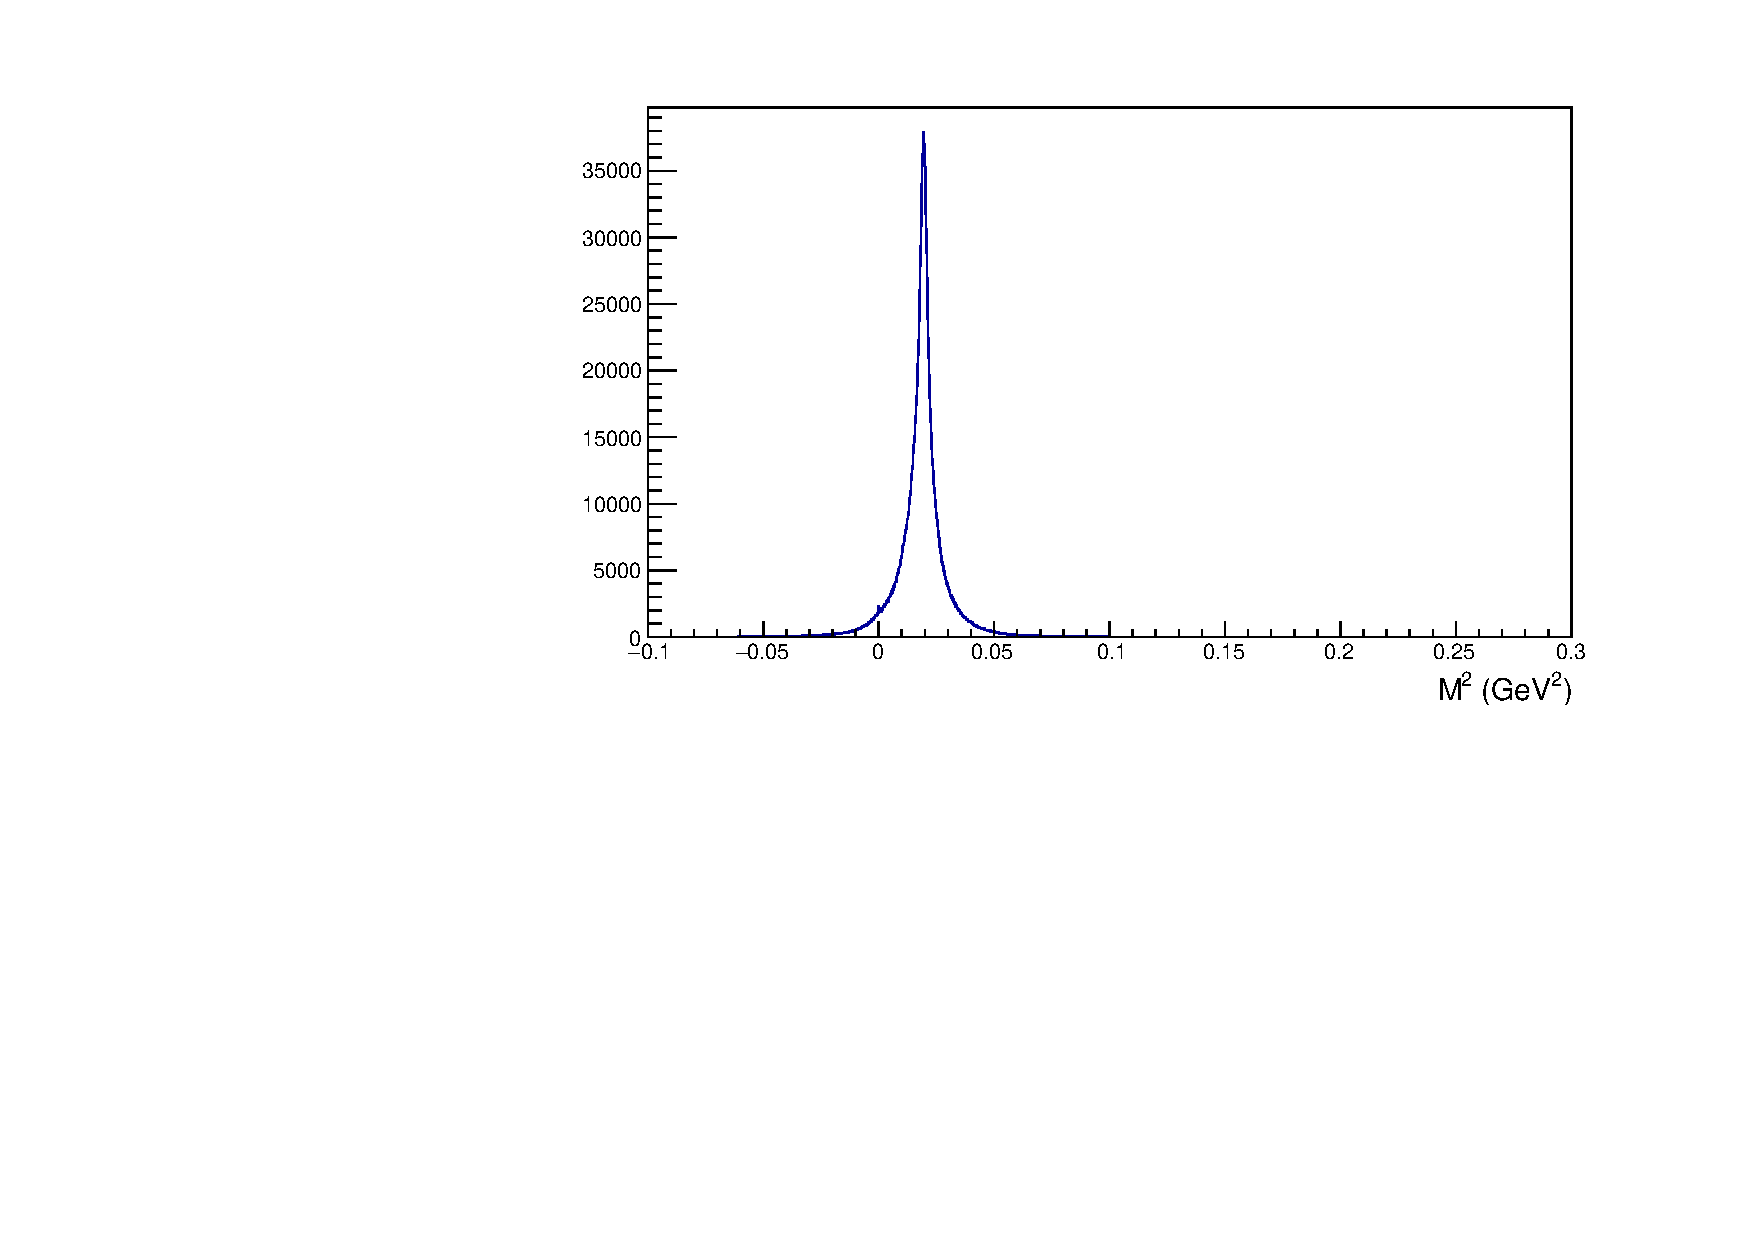
\includegraphics[width=0.6\textwidth]{figures/pid_mass2_pip.pdf} \\
    \caption{$M^2$ for the selected $\pi^+$ tracks}
    \label{fig:mass2_pip}
  \end{center}
\end{figure}

\subsubsection{Pion-Photon Timing}
The time at which each event took place was now compared to the timing of the photon measured by the tagger. This allowed the reduction of background and accurate knowledge of the photon energy corresponding to each event as required for the missing mass calculation. The photons within the coherent peak were first selected using a simple cut on the photon energy range. The upper limit of this range was the coherent peak setting, the lower limit was the photon energy at which the beam polarisation dropped to 20\%. The arrival time of these photons at the event vertex, $ t_\gamma$, was then calculated using the tagger time, $t_{TAG}$, and the distance the photon travels from the radiator to the event vertex along the axis of the beamline, $z$ :
$$
t_\gamma = t_{TAG} + \frac{z}{c}
$$
The $\pi^+$ time, $t_\pi$, the event vertex was then calculated as:
$$
t_\pi = t_{SC} - \frac{d}{c \beta_\pi}
$$
\begin{figure}[htb]
  \begin{center}
    \begin{tabular}{lr}
      \begin{minipage}{0.5\textwidth}
        \begin{flushleft}
          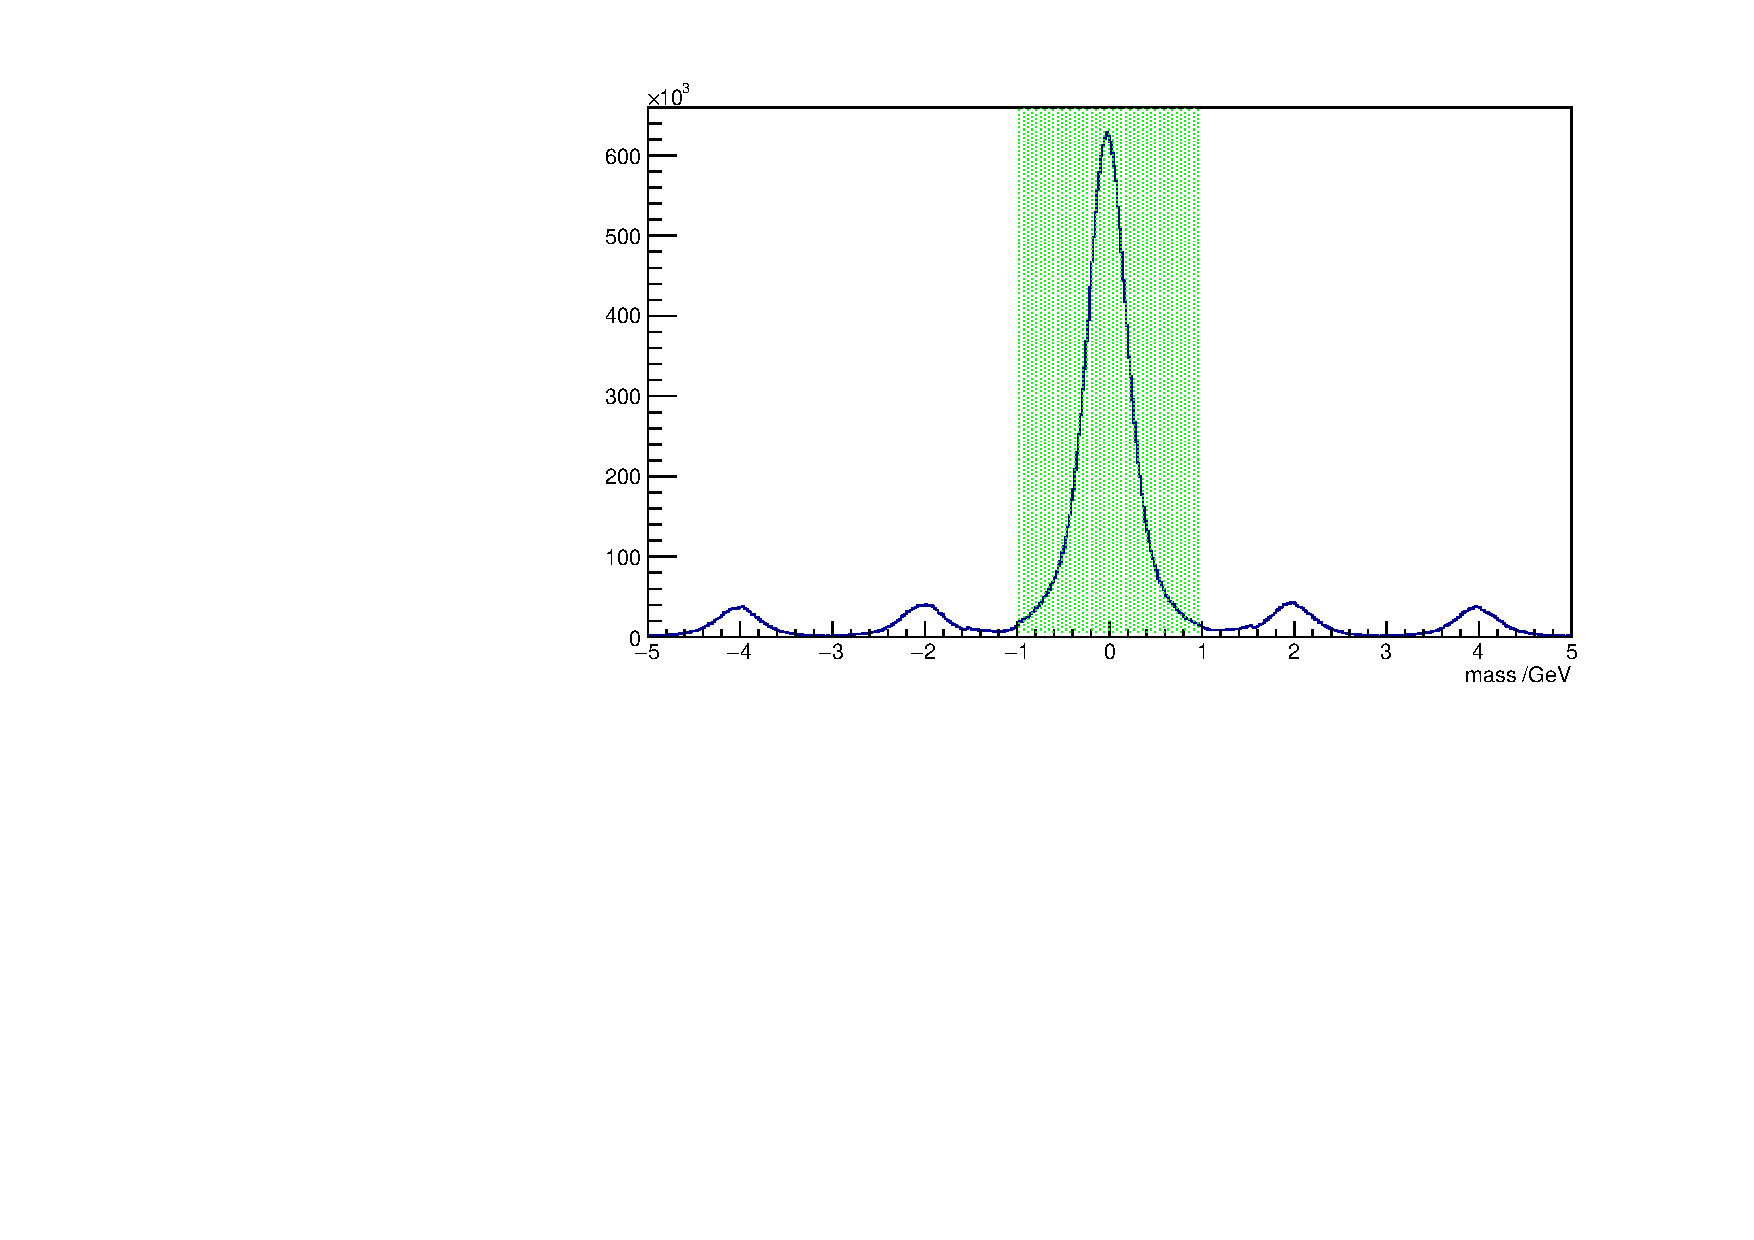
\includegraphics[width=0.95\textwidth]{figures/best_pion_photon_timing.pdf} \\
          \caption{Best Pion-photon timing}
          \label{fig:pion-photontiming}
        \end{flushleft}
        \end{minipage} &
        \begin{minipage}{0.5\textwidth}
        \begin{flushright}
          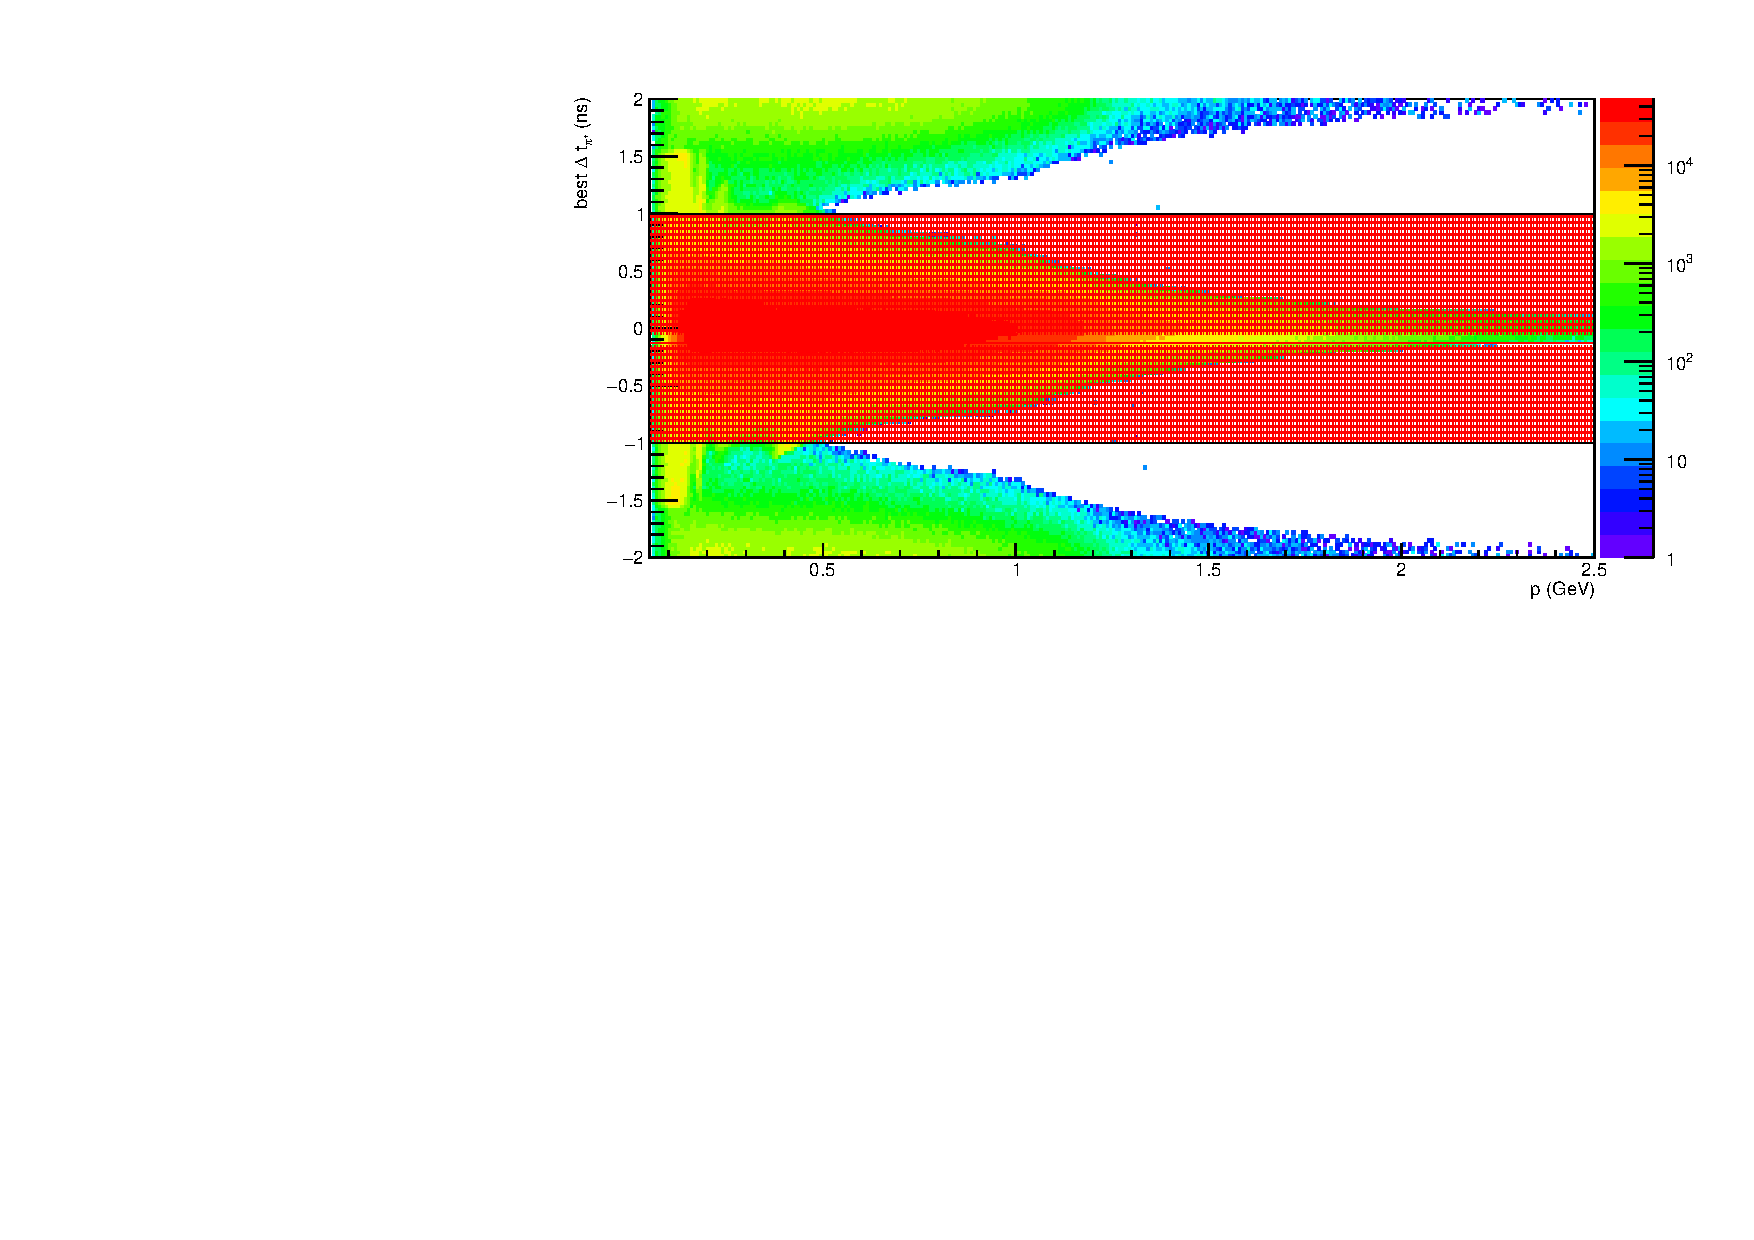
\includegraphics[width=0.95\textwidth]{figures/best_pion_photon_timing_vs_p.pdf} \\
          \caption{Best Pion-photon timing vs $\pi^+$ momentum}
          \label{fig:pion-photontiming_vsp}
        \end{flushright}
        \end{minipage}
    \end{tabular}
  \end{center}
\end{figure}
where $t_{SC}$ is the time recorded for the event by the Start Counter, $d$ is the distance between the event vertex and the hit position in the Start Counter  and $\beta_\pi = \sqrt{\frac{p^2}{m^2 + p^2}} $.  The event photon was defined as the photon whose vertex time is closest to the $\pi^+$ vertex time. Fig. \ref{fig:pion-photontiming} shows the time difference between these event photons and the $\pi^+$ vertex time, $\Delta t$ , with the majority of events having a time difference centred on zero (Fig. \ref{fig:pion-photontiming_vsp} shows the same quantity plotted vs the pion momentum). The smaller peaks to either side of the main peak correspond to photons from other beam buckets which were recorded during the time-window of the trigger for each event. These photons arising from neighbouring beam buckets were removed by setting the condition that 
\begin{enumerate}
\item $\Delta t$ must be within $1 ns$. 
\item One single photon in this timing region per event
\end{enumerate}


\subsubsection{Energy Loss Corrections}

The four-momentum of the $\pi^+$ is determined, in part, by the three-momentum obtained from the $\pi^+$ tracks in the drift chambers. This measured momentum does not take into account the energy losses of the particles as they pass through the target cell walls, mixing chamber and holding coil as well as the start counter before entering the drift chambers. As a result, the momentum of the $\pi^+$ can be up to $\sim 0.02 GeV/c$ higher than that measured, as shown in Figure 8.8.
The data were corrected for this loss in momentum using the ELOSS package [147] which was updated for g9a. This is the standard energy-loss correction software for CLAS experiments and can be applied to any charged particle with a mass greater than that of an electron. The target geometry, event vertex position, and particle four-momentum is input into ELOSS which then tracks back the flight path of the particle from the point at which it entered the Region 1 Drift Chambers to the event vertex. The path length of the particle in each of the materials it traverses is obtained allowing the energy lost in each material and hence the momentum lost by the particle to be calculated. The mass and energy of the $\pi^+$ were now recalculated using the energy-loss corrected values of momentum, the PDG value of $\pi^+$ mass and the measured value of beta (Equations 8.3 and 8.4). A new energy-loss corrected four-vector was therefore created for the $\pi^+$ which was then applied in the missing mass calculation described in the next section (See Fig. \ref{fig:eloss_comp} for an example of this correction).
\begin{figure}[htb]
  \begin{center}
    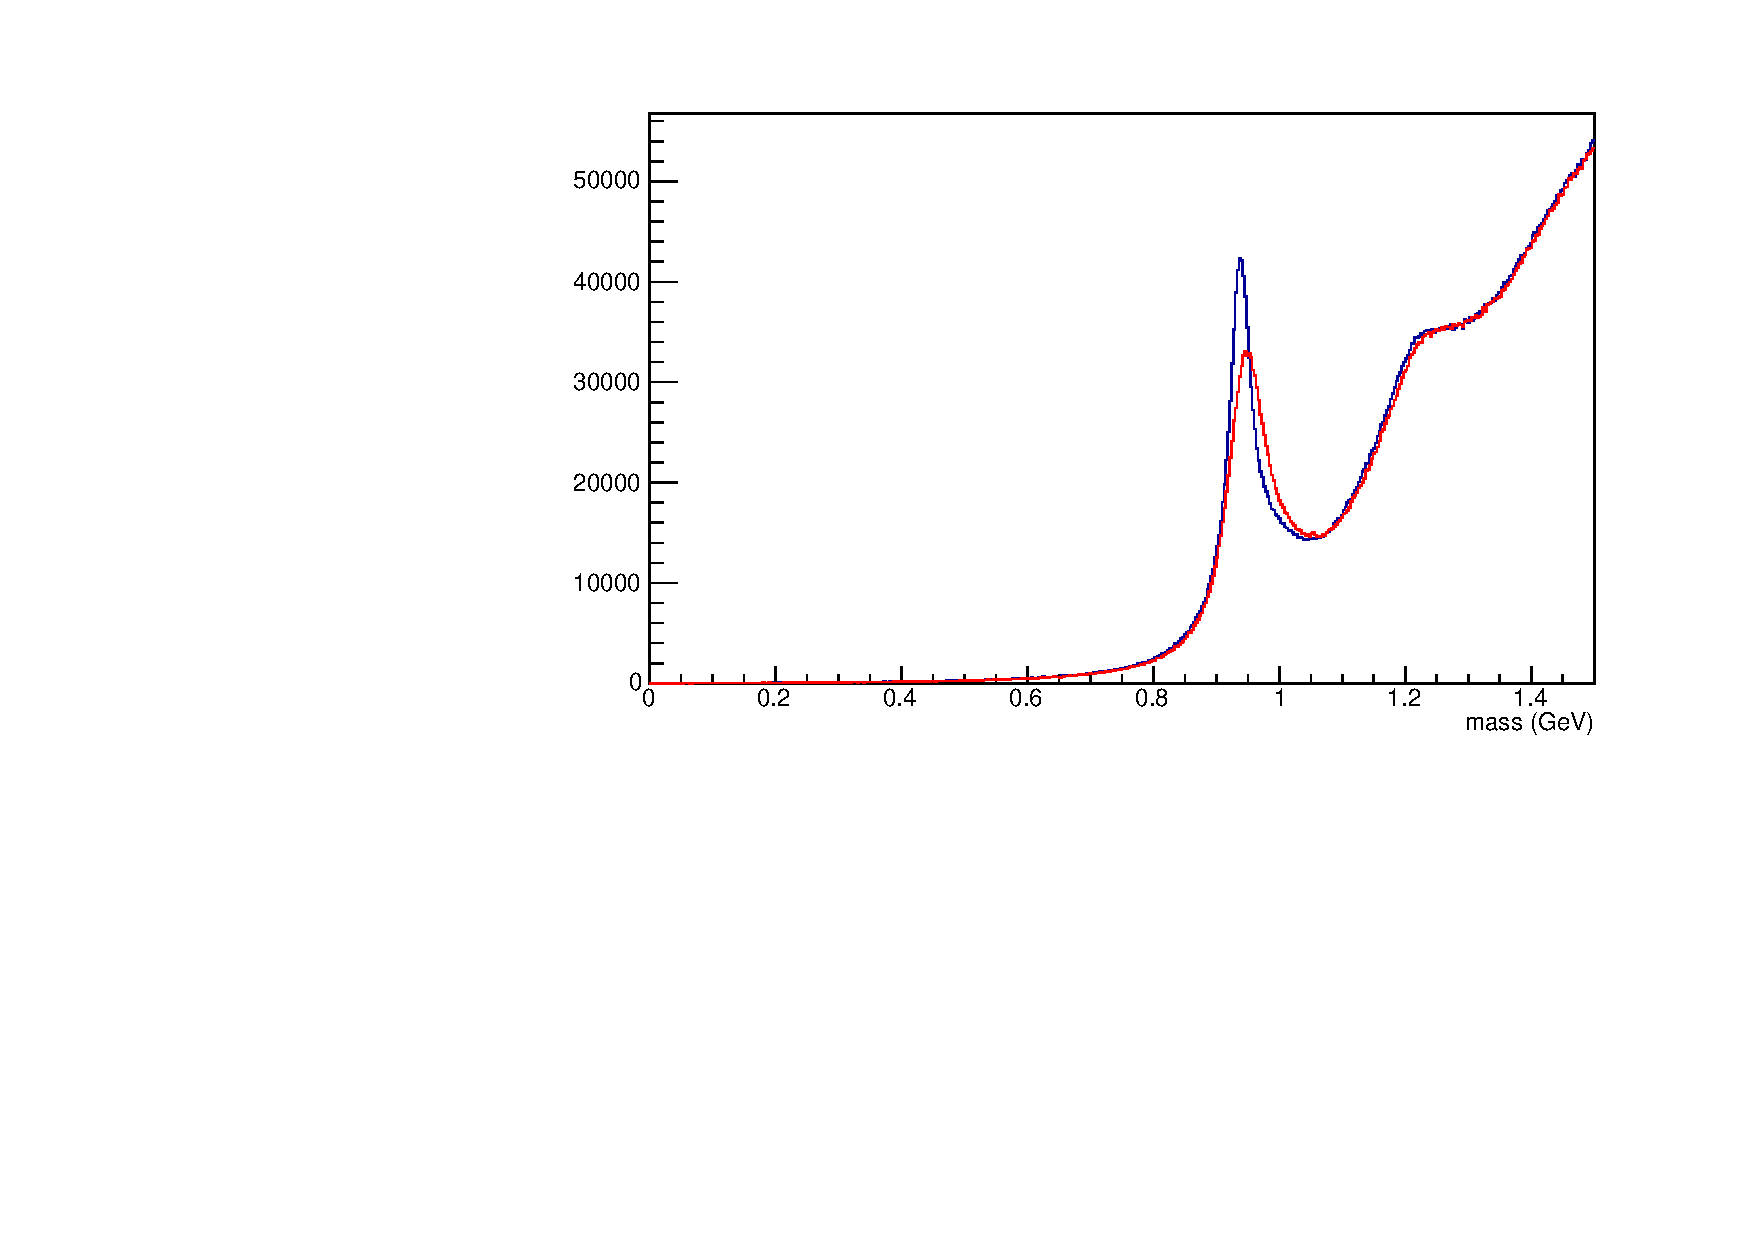
\includegraphics[width=0.6\textwidth]{figures/eloss_comp.pdf} \\
    \caption{Reconstructed Mass of the neutron before (red) and after eloss (blue)}
    \label{fig:eloss_comp}
  \end{center}
\end{figure}



